% COMPOSITE

\newpage

\subsection{Problem 8}

Jack and Jill ran up the hill at \SI{4.0}{m/s}. The horizontal component of Jill's velocity vector was \SI{2.5}{m/s}.

\setcounter{partcounter}{2}
\paragraph{Parts A-B}

What was the angle of the hill? Express your answer in degrees.

\begin{solution}
	I will draw a diagram for clarity.

	\begin{center}
		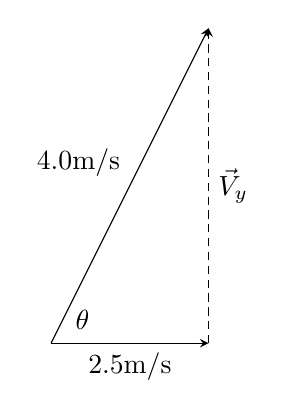
\begin{tikzpicture}[>=stealth]
			\draw[->] (0, 0) -- (2, 4) node[midway, above left] {\SI{4.0}{m/s}};
			\draw[->] (0, 0) -- (2, 0) node[midway, below] {\SI{2.5}{m/s}};
			\draw[->, densely dashed] (2, 0) -- (2, 4) node[midway, right] {$\vec{V}_y$};
			\draw (0.4, 0.3) node {$\theta$};
		\end{tikzpicture}
	\end{center}

	\begin{align*}
		\cos \left( \theta \right) &= \frac{2.5}{4.0} \\
		\theta &= \arccos \left( \frac{2.5}{4.0} \right) \\
		&\approx \SI{51.32}{\degree}
		.\end{align*}

	\begin{align*}
		\vec{V}_{y} &= \sin 4.0 \left( 51.32 \right) \\
		&\approx \SI{3.12}{\frac{m}{s}}
		.\end{align*}
\end{solution}
